\documentclass[11pt,a4paper]{article}
\usepackage[a4paper,margin=2.4cm]{geometry}
\usepackage{amsmath,amssymb,mathtools}
\usepackage{fontspec}
\usepackage{polyglossia}
\setmainlanguage{russian}
\setotherlanguage{english}
\setmainfont{Liberation Serif}
\setsansfont{Liberation Sans}
\setmonofont{Liberation Mono}
\newfontfamily\cyrillicfont[Ligatures=TeX]{Liberation Serif}
\newfontfamily\cyrillicfontsf[Ligatures=TeX]{Liberation Sans}
\newfontfamily\cyrillicfonttt{Liberation Mono}
\usepackage{booktabs}
\usepackage{enumitem}
\usepackage{graphicx}
\usepackage{float}
\usepackage[hidelinks]{hyperref}

\setlength{\parindent}{0pt}
\setlength{\parskip}{0.5em}
\emergencystretch=3em
\setlist{itemsep=0.15em,topsep=0.25em}

\newcommand{\G}{\mathcal{G}_k}
\newcommand{\norm}[1]{\lVert #1\rVert_2}
\newcommand{\E}{\mathbb{E}}
\DeclareMathOperator*{\argmin}{arg\,min}
\DeclareMathOperator{\diag}{diag}
\DeclareMathOperator{\Var}{Var}
\DeclareMathOperator{\sigm}{sigm}
\makeatletter\newcommand{\tabinput}[1]{\@@input #1 }\makeatother
\renewcommand{\figurename}{Рис.}
\renewcommand{\tablename}{Таблица}

\title{SGD против робастного SGD при неопределённости градиента\\[0.2em]\large Отчёт по домашнему мини-проекту}
\author{Егор Чулков, Владислав Дворников, Дарья Демешко}
\date{17 ноября 2026 г.}

\begin{document}
\maketitle

\noindent\textbf{Участники и вклад.}
Егор Чулков: [вклад].
Владислав Дворников: [вклад].
Дарья Демешко: [вклад].

\section*{Введение}

Мы исследуем робастный SGD (R-SGD). Вместо того чтобы доверять градиенту мини-батча $g_k$, он
делает шаг, хороший для любого градиента из эллипсоида $\G=\{g_k+S_k^{1/2}u:\norm u\le\rho\}$,
построенного по батчу. В разделе~1 выводятся шаг и его свойства. В разделе~2 описаны наша
реализация и проверки. В разделе~3 SGD и R-SGD сравниваются на логистической регрессии и небольшой
двухслойной сети. В разделе~4 объясняется, как мы сделали сравнение честным, а в разделе~5 обсуждаются
результаты. Код, результаты и команды для воспроизведения лежат в папке проекта (раздел~6).

\section{Вывод и интерпретация}

Ниже $S\succ0$, поэтому $S^{1/2}$ и $S^{-1/2}$ существуют, симметричны и $\sqrt{x^TSx}=\norm{S^{1/2}x}$.
Внутри одного шага пишем $g=g_k$, $S=S_k$, $\alpha=\alpha_k$.

\textbf{(a) Внутренний максимум.} При фиксированном $x$ по неравенству Коши — Буняковского
$\max_{\norm u\le\rho}(\mu+S^{1/2}u)^Tx=\mu^Tx+\max_{\norm u\le\rho}u^T(S^{1/2}x)=\mu^Tx+\rho\sqrt{x^TSx}$.
При $x\ne0$ максимум достигается в точке
\begin{equation*}
u^\star=\rho\,\frac{S^{1/2}x}{\norm{S^{1/2}x}},\qquad c^\star=\mu+\rho\,\frac{Sx}{\sqrt{x^TSx}} .
\end{equation*}
В локальной модели $f(\theta_k+d)\approx f(\theta_k)+\nabla f(\theta_k)^Td$ истинный градиент неизвестен.
Мы знаем только, что он правдоподобно лежит в $\G$, поэтому $x$ становится шагом $d$, а $\mu$ —
градиентом $g_k$. У линейной модели нет минимума, поэтому слагаемое $\norm d^2/(2\alpha_k)$ держит шаг
малым.

\textbf{(b) Эквивалентная задача.} Квадратичное слагаемое не зависит от $h$, поэтому по пункту (a)
\begin{equation*}
d_k=\argmin_d\varphi(d),\qquad \varphi(d)=g^Td+\rho\sqrt{d^TSd}+\frac{\norm d^2}{2\alpha}. \tag{2}
\end{equation*}
При $\rho=0$ функция $\varphi$ квадратичная с градиентом $g+d/\alpha$, поэтому $d_k=-\alpha g$, то
есть SGD. $\varphi$ — это линейная часть плюс выпуклая норма плюс $1/\alpha$-сильно выпуклая
квадратичная функция, поэтому она сильно выпукла и коэрцитивна. Значит, робастный шаг всегда
существует и единствен, хотя в $d=0$ функция $\varphi$ не дифференцируема. Умножив условие
оптимальности из (d) на $d^T$, получаем ещё $\norm{d_k}\le\alpha\norm{g_k}$: робастный шаг никогда не
длиннее шага SGD.

\textbf{(c) Нулевой шаг.} Покажем, что $d_k=0\iff g^TS^{-1}g\le\rho^2$ (условие (3)).
\begin{itemize}
\item Если (3) выполнено и $d\ne0$, по Коши — Буняковскому
$g^Td=(S^{-1/2}g)^T(S^{1/2}d)\ge-\sqrt{g^TS^{-1}g}\sqrt{d^TSd}\ge-\rho\sqrt{d^TSd}$. Отсюда
$\varphi(d)\ge\norm d^2/(2\alpha)>0=\varphi(0)$, то есть $d_k=0$.
\item Если $d_k=0$, возьмём $d=-tS^{-1}g$ и устремим $t\to0^+$. При $\kappa=\sqrt{g^TS^{-1}g}$
неравенство $\varphi(d)\ge0$ даёт $-t\kappa^2+\rho t\kappa+O(t^2)\ge0$, откуда $\kappa\le\rho$.
\end{itemize}
Условие (3) — то же самое, что $0\in\G$. Из него \textbf{не} следует $\nabla f(\theta_k)=0$: оно
говорит лишь, что данные не позволяют исключить нулевой градиент. Пример: $f=\tfrac12\theta^2$ в
точке $\theta_k=1$, $b=2$ наблюдения $3$ и $-1$. Тогда $g_k=1$, $s_k=4.004$ по формуле (4) и
$g_k^2/s_k=0.25\le1=\rho^2$, поэтому R-SGD стоит на месте, хотя $\nabla f=1$.

\textbf{(d) Условие оптимальности и изотропный случай.} При $d\ne0$ функция $\varphi$
дифференцируема, и так как она выпукла, шаг оптимален ровно тогда, когда
\begin{equation*}
g_k+\rho\,\frac{S_kd_k}{\sqrt{d_k^TS_kd_k}}+\alpha_k^{-1}d_k=0 .
\end{equation*}
При $S=sI$ это $(\alpha^{-1}+\rho\sqrt s/\norm d)\,d=-g$, значит, $d$ направлен вдоль $-g$.
Подставив $d=-t\,g/\norm g$, получаем $t=\alpha(\norm g-\rho\sqrt s)$; это положительно только при
$\norm g>\rho\sqrt s$. Иначе выполнено (3) и $d=0$. Вместе:
$d_k=-\alpha_k(1-\rho\sqrt s/\norm{g_k})_+\,g_k$. При $g_k=0$ имеем $\varphi(d)>0$ для всех $d\ne0$,
поэтому $d_k=0$.

В изотропном случае меняется только длина: $\norm{d}=\alpha(\norm g-\rho\sqrt s)_+$. В анизотропном
случае $d=-\alpha(I+\alpha\rho S/\tau)^{-1}g$, где $\tau=\sqrt{d^TSd}$. Направления с большей
неопределённостью сжимаются сильнее, поэтому меняется и направление: с ростом $\rho$ оно
поворачивается от $-g$ к $-S^{-1}g$.

\textbf{(e) Условное убывание.} Неравенство выполнено. При $d_k=0$ это очевидно. Иначе:
\begin{itemize}
\item по лемме о спуске $f(\theta_k+d)\le f(\theta_k)+\nabla f(\theta_k)^Td+\tfrac L2\norm d^2$;
\item так как $\nabla f(\theta_k)\in\G$, по (a) имеем $\nabla f(\theta_k)^Td\le g^Td+\rho\sqrt{d^TSd}$;
\item умножив условие из (d) на $d^T$, получаем $g^Td+\rho\sqrt{d^TSd}=-\norm d^2/\alpha$.
\end{itemize}
Значит, $f(\theta_k+d_k)\le f(\theta_k)-(\alpha_k^{-1}-L/2)\norm{d_k}^2$, и для убывания при
$d_k\ne0$ достаточно $\alpha_k<2/L$. Ключевое предположение — включение, и проверить его нельзя.
Если истинный градиент вне $\G$, величина $\nabla f^Td$ может быть положительной. Большее $\rho$ делает
включение вероятнее (примерно $P(\chi^2_p\le\rho^2)$, если бы $S_k$ была точной), но шаги становятся
короче, а нулевых шагов больше.

\section{Реализация и численные проверки}

\textbf{Наблюдения градиента и $S_k$.} Мы выбираем $b$ примеров с возвращением и считаем
градиенты отдельных примеров по явным формулам:
\begin{itemize}
\item логистическая регрессия: $u_i=(\sigm(t_i)-y_i)(a_i,1)$;
\item сеть: обратное распространение для каждого примера, $\delta=\sigm(t)-y$,
$\partial_{w_2}=\delta h$, $\partial_{b_1}=\delta\,w_2\odot(1-h^2)$, $\partial_{W_1}=\partial_{b_1}a^T$.
\end{itemize}
Центральные конечные разности совпадают с относительной ошибкой $<10^{-8}$ для обеих моделей. Шум
добавляется только к этим наблюдениям, $v_{k,i}=u_i+\sigma z_{k,i}$. По тем же $b$ наблюдениям мы
считаем $g_k$ и диагональную $S_k$ по формуле (4). Поскольку выбор с возвращением,
$\E\widehat s_{k,j}=\Var(g_{k,j})$ — дисперсия среднего по батчу.

\textbf{Решатель задачи (2).} Для диагональной $S$ из условия оптимальности
$d_j=-\alpha\,\tau g_j/(\tau+\alpha\rho s_j)$ с одной неизвестной $\tau=\sqrt{d^TSd}$, которая решает
\begin{equation*}
q(\tau)=\sum_j\frac{\alpha^2s_jg_j^2}{(\tau+\alpha\rho s_j)^2}=1 .
\end{equation*}
\begin{itemize}
\item $q$ убывает от $g^TS^{-1}g/\rho^2$ до $0$, поэтому корень существует ровно тогда, когда (3)
нарушено. Правило нулевого шага встроено в решатель: сначала проверяем (3) и при необходимости
возвращаем $d=0$.
\item Уравнение $q(\tau)^{-1/2}-1=0$ решаем методом Ньютона из $\tau=0$ со страховкой бисекцией на
$[0,\alpha\sqrt{g^TSg}]$. Эта функция вогнута (по Коши — Буняковскому), поэтому Ньютон монотонно
приближается к корню, а при $S=sI$ точен за один шаг.
\item Остановка: $|q^{-1/2}-1|\le10^{-14}$, или относительное изменение меньше $10^{-15}$, или не
более 100 итераций.
\item Итерация стоит $O(p)$, что мало по сравнению с $O(bp)$ на градиенты. Но в Python постоянные
накладные расходы делают обновление R-SGD в 3--4 раза медленнее обновления SGD.
\end{itemize}

\textbf{Проверки (пункт b).} На случайных тестовых задачах и на зашумлённой квадратичной функции из
раздела Illustration получили следующее.
\begin{center}
\small
\begin{tabular}{@{}lp{0.62\linewidth}@{}}
\toprule
Проверка & Результат \\
\midrule
$\rho=0$ & совпадает с SGD (1000/1000 задач и одинаковые траектории) \\
$\rho\to0$ & $\norm{d+\alpha g}$ стремится к 0 линейно по $\rho$ \\
Изотропная формула & макс.\ относительная ошибка $4.8\cdot10^{-12}$ на 10\,000 задач; Ньютон делает 1 итерацию \\
Нулевой шаг & совпадает с (3) во всех случаях, включая $\rho=(1\pm10^{-6})\sqrt{g^TS^{-1}g}$ \\
Условие 1(d) & невязка $\le1.0\cdot10^{-14}$; в среднем 4.4 итерации Ньютона (максимум 9) \\
Проверка через CVXPY & наша целевая функция ни разу не больше, чем у CVXPY \\
\bottomrule
\end{tabular}
\end{center}
На зашумлённой квадратичной функции R-SGD делал нулевые шаги и далеко от минимума, при $f$ до $2.9$
(старт $f=10$). Это происходит вдоль $\theta_1$, где градиент слабый, а шум сильный; это ровно
ситуация из пункта 1(c).

\textbf{Размер батча (пункт c).} $\widehat s_{k,j}$ оценивает $\Sigma_{jj}/b$, поэтому
неопределённость убывает как $1/b$. Но сама оценка шумная: её относительное стандартное отклонение
равно $\sqrt{2/(b-1)}$, то есть 141\% при $b=2$ и 53\% при $b=8$. Рис.~\ref{fig:batch} подтверждает обе
формулы.

Отсюда два следствия:
\begin{itemize}
\item при маленьком батче решения о нулевом шаге почти случайны;
\item при большом батче робастная поправка ($\propto\rho/\sqrt b$) исчезает, и R-SGD ведёт себя как
SGD.
\end{itemize}
Без возвращения $\widehat s$ завышала бы дисперсию в $n/(n-b)$ раз; мы проверили это численно.
Поэтому мы взяли $b=16$.

\begin{figure}[H]
\centering
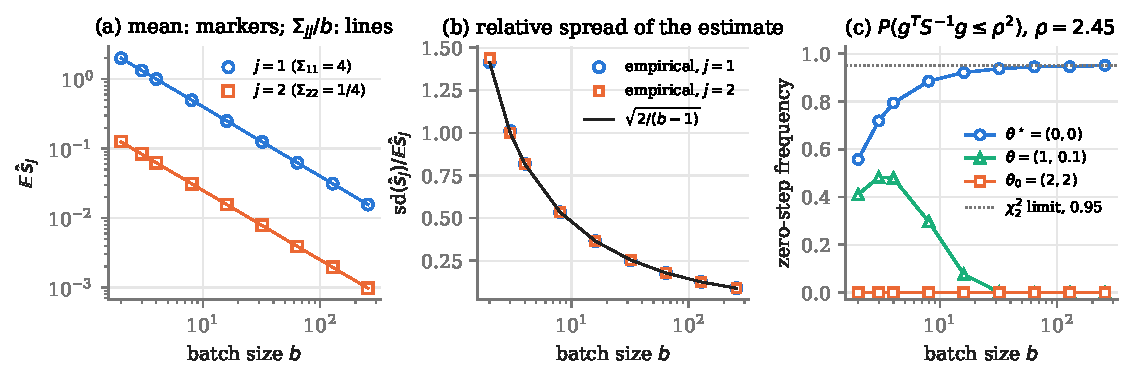
\includegraphics[width=0.92\linewidth]{fig/batch_size.pdf}
\caption{Зашумлённая квадратичная функция, $\sigma=1$, $20\,000$ батчей на каждое $b$. (a)
$\E\widehat s_j$ следует $\Sigma_{jj}/b$. (b) Её относительный разброс следует $\sqrt{2/(b-1)}$. (c) Доля
нулевых шагов при $\rho=2.45$ в трёх точках.}
\label{fig:batch}
\end{figure}

\textbf{Воспроизводимость (пункт d).} Всё считается во float64. Сиды берутся из \texttt{SeedSequence}
NumPy, с отдельными потоками для данных, инициализации, батчей и шума. SGD и R-SGD используют одни и
те же потоки (парные запуски). Шум затрагивает только наблюдаемые градиенты; целевая функция и все
оценки считаются на чистых данных. Подробности в разделе~6.

\section{Обязательные эксперименты}

\textbf{Условия (оба эксперимента).}
\begin{itemize}
\item Сбалансированные классы: 400 точек для обучения, 400 для валидации и 4000 для теста. Входы
стандартизуются по статистикам обучающей выборки.
\item Потери: BCE по логитам, вычисляется как \texttt{logaddexp(0,t)-y*t}, без регуляризатора;
класс определяется по $t>0$.
\item Бюджет: $b=16$, $K=500$ обновлений (логистическая регрессия) или $K=3000$ (сеть),
$\alpha_k=\alpha_0/\sqrt{1+k/50}$ для обоих методов.
\item Шум: $\sigma=c\,\gamma$ при $c\in\{0,1,4,16\}$, где $\gamma$ — среднеквадратичный градиент
примера в начальной точке ($0.50$ и $0.215$). Случай $c=0$ — без добавленного шума.
\item Радиус записываем как $\rho=r\sqrt p$, потому что вблизи минимума $g^TS^{-1}g\approx\chi^2_p$.
\end{itemize}

Настройки подобраны по валидации при $c=1$ и затем зафиксированы для всех уровней шума (раздел~4):
\begin{itemize}
\item логистическая регрессия: SGD $\alpha_0=0.3$; R-SGD $\alpha_0=1$, $\rho=1.30$;
\item сеть: SGD $\alpha_0=1$; R-SGD $\alpha_0=10$, $\rho=1.44$.
\end{itemize}
Все числа — среднее $\pm$ стандартное отклонение по 10 сидам оценки, у каждого свой набор данных.

\subsection{Эксперимент 1: логистическая регрессия}

Данные $a\mid y\sim\mathcal N((2y-1)(1,1)^T,I)$, модель $t=w^Ta+c$ ($p=3$), старт из
$\theta_0=0$. Модель верна для этих данных, поэтому лучшее возможное (байесовское) правило
$a_1+a_2>0$ даёт на наших тестовых выборках точность $0.923$.

\begin{figure}[H]
\centering
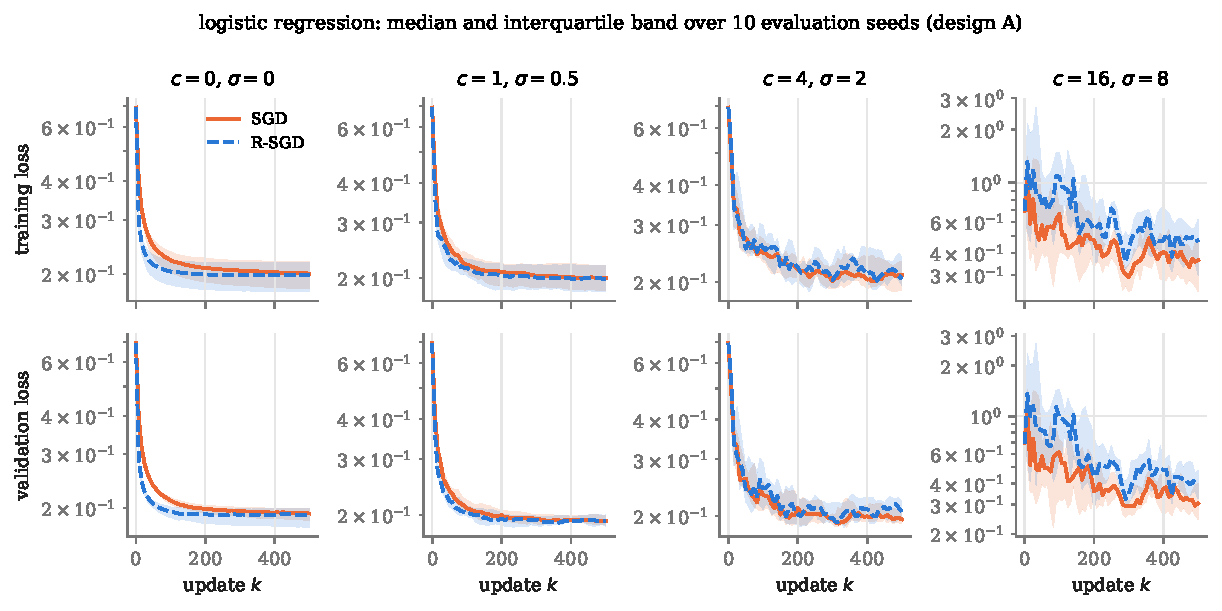
\includegraphics[width=\linewidth]{fig3/logreg_curves.pdf}
\caption{Логистическая регрессия: потери на обучении (сверху) и на валидации (снизу), медиана и
интерквартильная полоса по 10 сидам (подписи на английском).}
\label{fig:lr_curves}
\end{figure}

\begin{table}[H]
\centering
\footnotesize
\setlength{\tabcolsep}{3.5pt}
\begin{tabular}{@{}clccccc@{}}
\toprule
$c$ & метод & потери обуч. & потери тест & точность & нулевые шаги & время, мс (мкс/обн.) \\
\midrule
\tabinput{tabs3/tab_lr_main.tex}
\bottomrule
\end{tabular}
\caption{Логистическая регрессия, итоговые результаты (среднее $\pm$ sd по 10 сидам; 8000 вычислений
градиента за запуск у обоих методов).}
\label{tab:lr}
\end{table}

\begin{figure}[H]
\centering
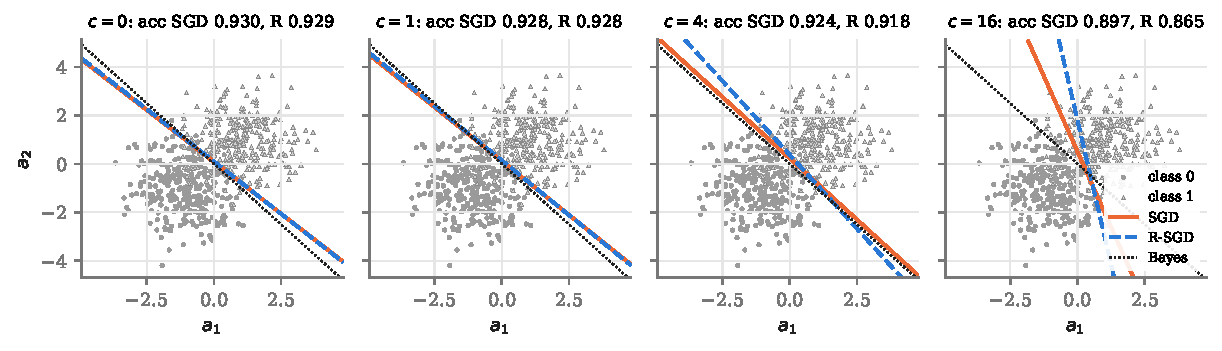
\includegraphics[width=\linewidth]{fig3/logreg_boundaries.pdf}
\caption{Границы решения для сида оценки 0 (пунктир — байесовское правило).}
\label{fig:lr_bound}
\end{figure}

Результаты:
\begin{itemize}
\item Оба метода достигают байесовской точности при $c\le4$, и границы почти совпадают.
\item При малом шуме у R-SGD немного меньше потери, примерно на $0.002$--$0.003$, но точность та же.
\item При сильном шуме ($c=16$) зафиксированная настройка R-SGD хуже: потери на тесте $+0.095$, SGD
лучше в 8/10 сидов.
\item R-SGD делает 18--33\% нулевых шагов, но всё равно сходится, так как $p=3$.
\end{itemize}

\subsection{Эксперимент 2: двухслойная сеть}

Данные — зашумлённые полуокружности. Модель $t=w_2^T\tanh(W_1a+b_1)+b_2$ с 8 скрытыми нейронами
($p=33$). Инициализация: $W_1\sim\mathcal N(0,\tfrac12)$, $w_2\sim\mathcal N(0,\tfrac18)$, нулевые
смещения; оба метода стартуют из одной и той же $\theta_0$.

\begin{figure}[H]
\centering
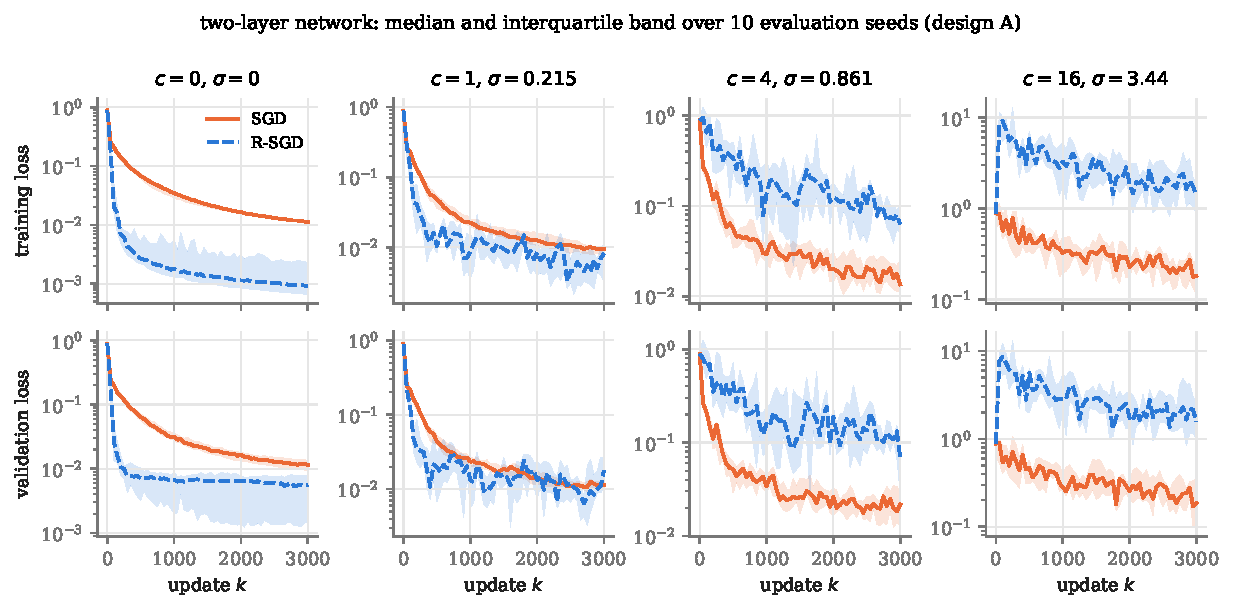
\includegraphics[width=\linewidth]{fig3/mlp_curves.pdf}
\caption{Двухслойная сеть: потери на обучении (сверху) и на валидации (снизу), медиана и
интерквартильная полоса по 10 сидам.}
\label{fig:mlp_curves}
\end{figure}

\begin{table}[H]
\centering
\footnotesize
\setlength{\tabcolsep}{3.5pt}
\begin{tabular}{@{}clccccc@{}}
\toprule
$c$ & метод & потери обуч. & потери тест & точность & нулевые шаги & время, мс (мкс/обн.) \\
\midrule
\tabinput{tabs3/tab_mlp_main.tex}
\bottomrule
\end{tabular}
\caption{Двухслойная сеть, итоговые результаты (среднее $\pm$ sd по 10 сидам; 48\,000 вычислений
градиента за запуск).}
\label{tab:mlp}
\end{table}

\begin{figure}[H]
\centering
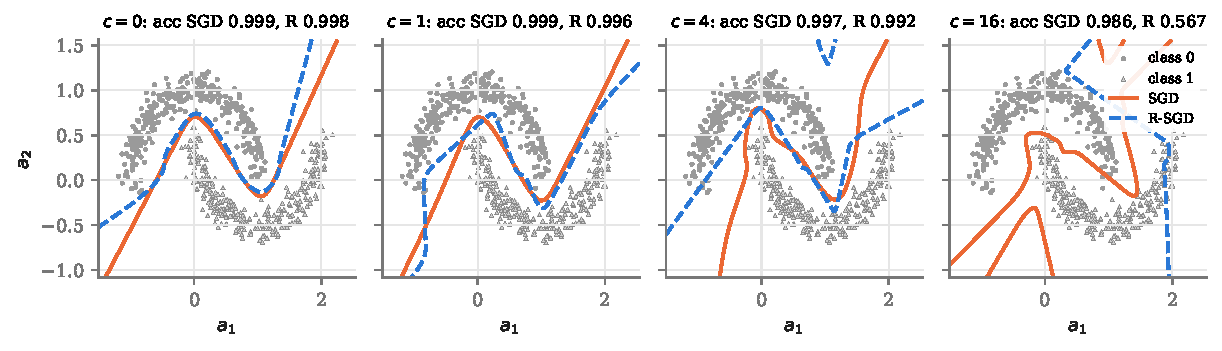
\includegraphics[width=\linewidth]{fig3/mlp_boundaries.pdf}
\caption{Границы решения для сида оценки 0.}
\label{fig:mlp_bound}
\end{figure}

Результаты:
\begin{itemize}
\item Без шума R-SGD оптимизирует гораздо быстрее: потери на обучении $0.0019$ против $0.0110$
(10/10 сидов). Точность та же, $0.998$.
\item С шумом зафиксированная настройка R-SGD хуже. При $c=16$ 8 из 10 запусков заканчиваются с
потерями выше начальных $\log2$, и граница на рис.~\ref{fig:mlp_bound} разваливается.
\item При выбранном $\rho$ нулевых шагов нет; проблема в большом шаге обучения (раздел~5).
\end{itemize}

\subsection{Совпадают ли ранжирования по оптимизации и по предсказанию?}

Не всегда.
\begin{itemize}
\item При малом шуме меньшие потери на обучении обычно означали и меньшие потери на тесте, но не
более высокую точность: знак разности потерь на обучении предсказал разность точностей лишь в 3--5
из 10 сидов.
\item При большом шуме все ранжирования совпадают, SGD лучше в 7--10 из 10 сидов.
\end{itemize}

\section{Честная настройка и оценка}

\textbf{Бюджеты.} Оба метода используют один батч, одно число обновлений и одно расписание, поэтому
тратят одинаковое число вычислений градиента ($bK$). Время замеряется только на обновлениях.

\textbf{Настройка.}
\begin{itemize}
\item Сетки: $\alpha_0\in\{0.1,0.3,1,3,10,30\}$ для обоих методов и
$r=\rho/\sqrt p\in\{0,0.25,0.5,0.75,1,1.25\}$ для R-SGD; $r=0$ — обычный SGD.
\item Критерий: средние потери на валидации в конце обучения по 3 сидам настройки при $c=1$.
Тестовые данные не использовались.
\item Бюджеты поиска: 18 запусков для SGD и 108 для R-SGD.
\item Ни одно выбранное значение не лежит на краю сетки (рис.~\ref{fig:tuning}).
\item По поверхностям видно, что больший $\alpha_0$ компенсируется бо́льшим $r$: оба управляют длиной
шага.
\end{itemize}

\begin{figure}[H]
\centering
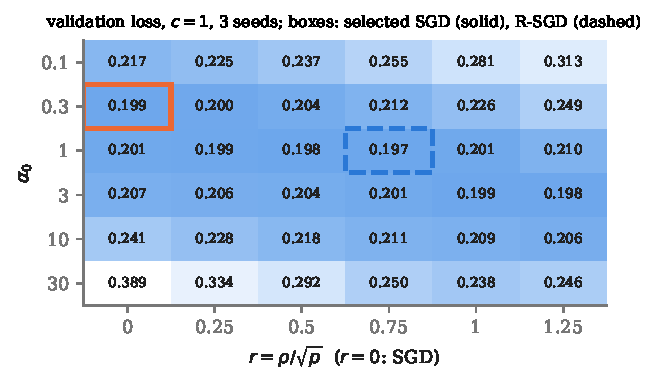
\includegraphics[width=0.48\linewidth]{fig3/logreg_tuning.pdf}\hfill
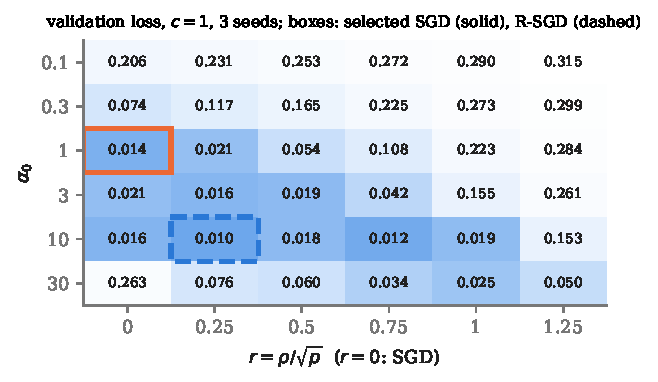
\includegraphics[width=0.48\linewidth]{fig3/mlp_tuning.pdf}
\caption{Потери на валидации при настройке (слева — логистическая регрессия, справа — сеть); рамки
отмечают выбранные настройки.}
\label{fig:tuning}
\end{figure}

\textbf{Сиды и погрешности.} Мы использовали 10 сидов оценки с парными запусками: одни и те же
данные, инициализация, батчи и шум для обоих методов. Погрешности — стандартные отклонения по этим
сидам. Чтобы разделить источники разброса, мы также сделали 10 сидов на одном фиксированном наборе
данных. Для логистической регрессии при малом шуме разброс в основном идёт от набора данных: на
фиксированных данных стандартное отклонение потерь на тесте в 2--7 раз меньше. Для сети
инициализация важна не меньше, чем данные. Неудачных запусков не было (бесконечные потери или
превышение начальных в 50 раз).

\textbf{Чувствительность и длина шага.} Мы меняли $r$ при $\alpha_0$ из настройки SGD (5 сидов,
рис.~\ref{fig:sens}). Чтобы проверить, не сводится ли выигрыш к более короткому шагу, мы также
запускали SGD с $\alpha_0$, умноженным на среднее отношение шагов R-SGD
$\overline{\norm{d_k}/(\alpha_k\norm{g_k})}$ (таблица~\ref{tab:matched}).

\begin{figure}[H]
\centering
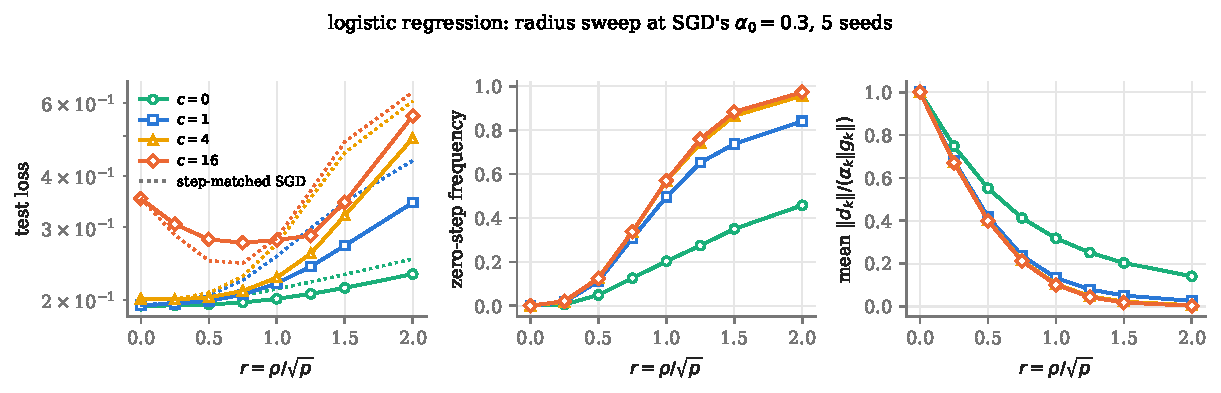
\includegraphics[width=\linewidth]{fig3/logreg_sensitivity.pdf}\\[0.3em]
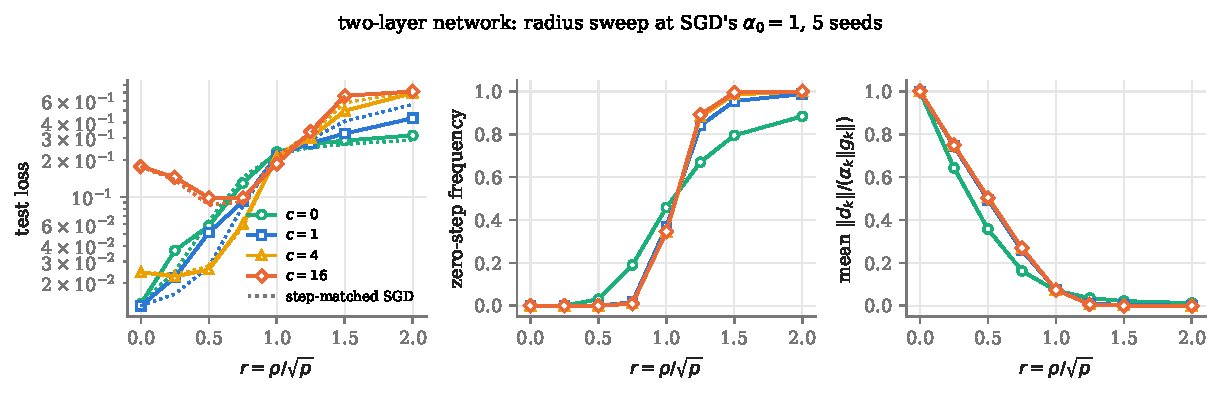
\includegraphics[width=\linewidth]{fig3/mlp_sensitivity.pdf}
\caption{Перебор радиуса для логистической регрессии (сверху) и сети (снизу). Слева: потери на тесте
R-SGD (сплошные) и SGD с той же длиной шага (пунктир). В центре: доля нулевых шагов. Справа: среднее
отношение шагов.}
\label{fig:sens}
\end{figure}

\begin{table}[H]
\centering
\small
\begin{tabular}{@{}lcccccc@{}}
\toprule
& $c$ & отн.\ шага & R-SGD & SGD, тот же шаг & SGD (настр.) & R-SGD лучше \\
\midrule
Логистическая & 0 & 0.30 & 0.1932 & 0.1951 & 0.1951 & 5/10 \\
Логистическая & 1 & 0.22 & 0.1949 & 0.1976 & 0.1955 & 9/10 \\
Логистическая & 4 & 0.22 & 0.2083 & 0.2029 & 0.2031 & 2/10 \\
Логистическая & 16 & 0.22 & 0.4297 & 0.2883 & 0.3343 & 1/10 \\
Сеть & 0 & 0.59 & 0.0082 & 0.0065 & 0.0133 & 4/10 \\
Сеть & 1 & 0.74 & 0.0246 & 0.0164 & 0.0126 & 2/10 \\
Сеть & 4 & 0.74 & 0.1149 & 0.1479 & 0.0246 & 7/10 \\
Сеть & 16 & 0.74 & 1.9569 & 1.2917 & 0.2241 & 2/10 \\
\bottomrule
\end{tabular}
\caption{Потери на тесте R-SGD против SGD с той же средней длиной шага (последний столбец — сиды, где
R-SGD лучше такого SGD).}
\label{tab:matched}
\end{table}

В большинстве случаев SGD с той же длиной шага не хуже R-SGD или лучше. Единственное явное
исключение — логистическая регрессия при $c=1$, где R-SGD выигрывает в 9/10 сидов. Радиусы
$r\gtrsim1$ дают много нулевых шагов: сеть застревает на точности $0.5$--$0.9$.

\section{Критический анализ}

\textbf{(a) Когда R-SGD помогает?}
\begin{itemize}
\item В наших экспериментах — немного и только по потерям: при малом шуме в логистической регрессии
R-SGD обошёл и SGD, и SGD с той же длиной шага.
\item Там его сжатие работает как адаптивное уменьшение шага: слабое в начале, когда градиенты
большие и надёжные, и сильное вблизи минимума.
\item Большой выигрыш сети при $c=0$ объясняется длиной шага: настройка выбрала в 10 раз больший
$\alpha_0$, и SGD с тем же эффективным шагом справляется так же.
\item При сильном шуме R-SGD был хуже. Когда добавленный шум доминирует, $S_k\approx sI$ и
$\norm{g_k}^2\approx ps$, поэтому по 1(d)
\begin{equation*}
\frac{\norm{d_k}}{\alpha_k\norm{g_k}}\approx1-\frac{\rho}{\sqrt p}.
\end{equation*}
Для сети мы измерили $0.75$, $0.50$, $0.27$ при $r=0.25$, $0.5$, $0.75$.
\item То есть R-SGD тогда — это просто SGD с более коротким шагом, причём самые большие (самые
шумные) градиенты он сжимает меньше всего. Настроенный SGD он там обыграть не может.
\end{itemize}

\textbf{(b) Радиус, ковариация и шаг обучения.}
\begin{itemize}
\item $\alpha$ и $\rho$ вместе управляют длиной шага (см.\ диагонали при настройке).
\item Решение о нулевом шаге зависит только от $\rho$ и $S_k$, но не от $\alpha$.
\item $S_k$ ведёт себя как (шум $+$ дисперсия выбора)$/b$, поэтому одно и то же $\rho$ означает
разную робастность при разных $b$ и уровнях шума.
\item Нулевые шаги возникают везде, где градиент мал по сравнению со своим шумом, а не только в
минимуме. На зашумлённой квадратичной функции эта область вытянута вдоль $\theta_1$.
\item При сильном шуме $g^TS^{-1}g$ выглядит одинаково везде (около $p(b-1)/(b-3)$), поэтому при
$r\gtrsim1$ нулевые шаги происходят почти всегда. В сети при $r=2$ и $c\ge4$ параметры вообще не
сдвинулись.
\end{itemize}

\textbf{(c) Означают ли меньшие потери на обучении более высокую точность?} Нет. В сети R-SGD
достиг в $5.8$ раза меньших потерь на обучении при той же точности. В логистической регрессии оба
метода уже на байесовской точности. Меньшая кросс-энтропия здесь в основном означает более уверенные
предсказания на уже правильно классифицированных точках. Только при сильном шуме, когда портится сама
граница, потери и точность согласовывались.

\textbf{(d) Ограничения и следующий эксперимент.}
\begin{itemize}
\item Мы настраивали всего по 3 сидам на одном уровне шума, и у R-SGD была большая сетка. Его
выбранная настройка для сети не повторила своё преимущество из настройки при оценке (потери на
валидации $0.023$ против $0.011$ при $c=1$).
\item Добавленный шум был изотропным — это ровно тот случай, когда R-SGD сводится к укороченному
шагу SGD.
\item $S_k$ диагональная, задачи маленькие, а время мерили в чистом Python.
\end{itemize}
\emph{Следующий эксперимент:} добавлять шум только в часть параметров, например в веса первого слоя,
и настраивать оба метода отдельно на каждом уровне шума с равными бюджетами. Тогда $S_k$ далека от
$sI$, и можно проверить, обыгрывает ли покоординатное сжатие R-SGD лучший шаг SGD.

\section{Воспроизводимость}

Папка проекта содержит:
\begin{itemize}
\item \texttt{Code/}:
  \begin{itemize}
  \item \texttt{rsgd.py}: оценка, решатель и оракулы градиента;
  \item \texttt{checks\_section2.py}: проверки раздела~2, около 20\,с;
  \item \texttt{sim3\_core.py}, \texttt{sim\_section3.py}: разделы~3--4 (около 3 минут);
  \item \texttt{make\_tables3.py}: таблицы.
  \end{itemize}
\item \texttt{Results/}: все числа в JSON и NPZ.
\item \texttt{Report/}: этот отчёт, его исходник LaTeX и наши более подробные заметки.
\end{itemize}
Главные сиды — 20261117 (раздел~2) и 20261118 (разделы~3--4). Использовались Python 3.13, NumPy 2.5.3,
SciPy 1.18.1 и Matplotlib 3.11.2.

\begin{thebibliography}{9}
\small
\bibitem{bental} A.~Ben-Tal, L.~El Ghaoui, A.~Nemirovski. \emph{Robust Optimization}. Princeton
University Press, 2009.
\bibitem{bottou} L.~Bottou, F.~E.~Curtis, J.~Nocedal. Optimization methods for large-scale machine
learning. \emph{SIAM Review} 60(2):223--311, 2018.
\bibitem{boyd} S.~Boyd, L.~Vandenberghe. \emph{Convex Optimization}. Cambridge University Press, 2004.
\bibitem{more} J.~J.~Moré, D.~C.~Sorensen. Computing a trust region step. \emph{SIAM J.\ Sci.\ Stat.\
Comput.} 4(3):553--572, 1983.
\bibitem{nocedal} J.~Nocedal, S.~J.~Wright. \emph{Numerical Optimization}, 2nd ed. Springer, 2006.
\end{thebibliography}

\end{document}
